\chapter{État de l'art}
\label{ch:etat_art}

\section{Protocoles de consensus}

Dans une blockchain, un protocole de consensus est un algorithme permettant de mettre l'ensemble des noeuds du réseau d'accord sur une version de la blockchain, ceci en tenant compte du fait que certains noeuds peuvent être malveillants.

Dans une structure centralisée, comme une banque par exemple, les transactions sont vérifiées par la banque elle-même, il est donc difficile de forger de fausses transactions puisque ces dernières sont vérifiées pas une entité centrale. Or, dans une structure décentralisée comme une blockchain, tout le monde peut se joindre au réseau et soumettre des blocs avec des transactions. Certains nœuds peuvent transmettre aux autres nœuds des blocs avec des transactions invalides et commettre des actes frauduleux comme de la double dépense.

Il nous faut donc un algorithme permettant de synchroniser tous les nœuds sur une version identique de la blockchain afin de garantir l'authenticité de tous les blocs qu'elle contient et empêcher qu'une même entité contrôle toute la chaîne de blocs. Ainsi, un protocole de consensus va permettre de déterminer quel nœud va pouvoir effectuer les calcules ou actions nécessaires afin d'ajouter un nouveau bloc à la chaîne. Dans le but de motiver les nœuds à agir de manière honnête, le réseau les récompense le plus souvent lors de la création d'un nouveau bloc avec une certaine quantité de cryptomonnaie. 

Tous les autres nœuds doivent alors se synchroniser et travailler sur la chaîne de blocs la plus longue s'il y a plusieurs branches disponibles. Le but étant que la chaîne de blocs honnête grandisse plus rapidement que d'autres chaînes isolées ou frauduleuses.

\subsection{Proof of work}
\label{consensus:pow}

\textit{Proof of work} (PoW, preuve de travail en français) est un des tout premier protocole de consensus créé et est aujourd'hui un des plus utilisé. Il a au début été développé afin se prémunir des spams d'e-mail. Il a, en 2009, été adapté pour les blockchains par Satoshi Nakamoto en créant le \textbf{Bitcoin}.

Le protocole \textit{proof of work} utilise des ordinateurs appelés mineurs pour vérifier les blocs en résolvant des puzzles mathématiques. La résolution de ses puzzles requiert une grande puissance de calcule et une grande quantité d'énergie.

Techniquement, les mineurs utilisent des fonctions de hachage cryptographiques. Pour simplifier le processus, ces derniers doivent hacher l'ensemble des données du dernier bloc ($Bloc_n$) et un nombre ($p$) qu'ils peuvent choisir. Ce nombre est appelé la \textbf{preuve de travail}. Ci-dessous, un exemple du calcul réalisé par un mineur :

\begin{equation*}
    H = \textsf{SHA256}(\textsf{Bloc}_n \| p)
\end{equation*}

L'objectif est que le hash final $H$ commence par un certain nombre de 0. Ce nombre est fixé par le réseau. Comme les fonctions de hachage ne permettant pas de retrouver les données fournies en entrée à partir de la sortie, il n'y a pas d'autre moyen que de tester toutes les entrées possible jusqu'à ce que le hash commence par le bon nombre de 0. Ainsi le mineur va modifier la preuve de travail $p$ jusqu'à ce que le hash $H$ remplisse les conditions de la blockchain. 

Le nombre de 0 demandé en sortie est ce que l'on appelle la \textbf{difficulté} de la preuve de travail car plus il y a de 0 à la suite, plus il faudra de temps au mineur pour trouver la preuve de travail correspondante. Ce nombre de 0 est automatiquement définit par le réseau et est adapté à la puissance de calcul globale. C'est-à-dire que si la puissance augmente parce que de nouveaux mineurs ont rejoint le réseau, alors la difficulté augmentera également. Ceci afin de maintenir le temps de création d'un bloc à environ 10 minutes. Si des mineurs viendraient à quitter le réseau, il y aurait moins de puissance de calcul disponible, la difficulté sera alors revue à la baisse.

\subsection{Proof of stake, delegated proof of stake}
\label{consensus:pos}

Le protocole de \textit{proof of stake} (PoS, preuve d'enjeu en français) est le deuxième protocole le plus utilisé dans les blockchains actuelles. Il fonctionne sur un principe totalement différent que PoW car il ne requiert pas de puissance de calcul particulière ce qui en fait un bonne alternative en terme d'énergie. La cryptomonnaie Ether du réseau Ethereum est en train d'effectuer une migration vers du \textit{proof of stake} en 2021.

\textit{Proof of stake} fonctionnement sur le principe de staking. C'est-à-dire allouer une certaine quantité de cryptomonnaie au réseau. Cette monnaie bloquée appartient toujours à l'utilisateur mais ne peut plus être utilisée. Les nouveaux blocs seront créés par les utilisateurs qui mise le plus de jetons dans le réseau. Si ces personnes ne respectent pas leur engagement de contribuer au réseau de manière légitime, elle perdraient leur mise ce qui potentiellement ruinerait ces derniers. 

Avec cette architecture, pour pouvoir effectuer un acte de double dépense, il faudrait posséder et bloquer plus de la moitié de tous les jetons misés sur le réseau pour le contrôler ce qui rend ces attaques difficiles. Mais le fait que \textit{PoS} ne requiert pas de puissance de calcule amène d'autres problèmes qui n'existaient pas avec \textit{PoW} comme par exemple le problème du Nothing-to-stake.

Un autre problème que l'on peut remarquer avec ce protocole est que ce sont toujours les utilisateurs qui mise le plus qui sont prioritaires pour ajouter des blocs à la blockchain ce qui peut rendre le protocole trop centralisé alors que l'on recherche plutôt l'inverse.

Pour palier à ce problème, on a créé le \textit{delegated proof of stake}. Le principe est qu'on utilise cette fois-ci un système de vote dans lequel chaque utilisateur possède un nombre de voix proportionnel à la quantité de monnaie misée dans le réseau. Le système de vote varie en fonction des implémentations. Cela rend le protocole plus démocratique et ainsi ce ne sont pas toujours les mêmes entités qui ajoutent des blocs.

\subsection{Proof of authority, proof of reputation}
\label{consensus:poa}

\emph{Proof of authority} (PoA) est un algorithme proposé par un des cofondateur d'Ethereum, Gavin Wood. Ce protocole se base lui sur la \textbf{réputation} des entités qui valident les blocs. A la différence du \hyperref[consensus:pos]{\emph{proof of stake}} qui se sert de la monnaie, \emph{PoA} met en valeur l'identité des validateurs qui sont sélectionnés comme entités de confiance.

Il y a ainsi un nombre limité de validateurs ce qui rend le réseau plus évolutif et efficace qu'un système avec du \hyperref[consensus:pow]{proof of work} ou proof of stake car le consensus peut être atteint plus rapidement.

\emph{Proof of authority} est un protocole qui se porte particulièrement bien au \textbf{blockchains privées} permettant aux entreprise d'utiliser pleinement la technologie de la blockchain avec une architecture centralisée. En effet, l'aspect décentralisé du \emph{PoW} et \emph{PoS} peut ne pas convenir à certaines sociétés. D'un autre côté, ce protocole ne s'adapte pas très bien au blockchain publique du fait de sa centralisation. Centralisation que les utilisateurs des blockchains cherchent à évité pour des raisons de confidentialité (politique) et de sécurité (pannes, attaques).

On peut voir le \emph{PoA} comme un renoncement à la décentralisation dans un but d'efficacité mais ce mécanisme n'est pas vu de la même manière par tous. Notamment critiqué à cause des risques de corruption possibles si les identités des validateurs sont connus. En effet, un concurrent pourrait influencer les validateurs pour compromettre le réseau de l'intérieur.

En conclusion, \emph{PoA} est une bonne alternative au \emph{PoW} et \textit{PoS} pour les \textbf{blockchains privées} d'entreprise souhaitant utiliser ses technologies.

\subsection{Proof of space, proof of space-time}
\label{consensus:pospace}
% TODO: Add details

\emph{Proof of space} est un protocole ressemblant à \hyperref[consensus:pow]{proof of work} à la différence qu'au lieu de réaliser des puzzles mathématiques, les mineurs appelé farmers vont réalisés des preuves cryptographiques en allouant de l'\textbf{espace disque inutilisé} au réseau. Il est également appelé \emph{proof of capacity}. Ce principe permet de créer des preuves et valider les blocs rapidement avec un coût énergétique beaucoup plus faible que \emph{proof of work}. Ainsi on utilise la capacité de stockage comme ressource au lieu de la puissance de calcul.

Cependant, comme les vérifications peuvent être faites très rapidement comparé au Bitcoin où il faut trouver la solution au puzzle qui prend obligatoirement du temps, des nouvelles attaques apparaissent. Par exemple, un attaquant peut valider un grande quantité de blocs à la suite et les soumettre au réseau d'un seul coup. Chose qui n'est pas possible avec \emph{proof of work} puisque qu'il faut nécessairement trouver la preuve de travail avant de vérifier le suivant. Or trouver la preuve de travail prend du temps, beaucoup plus qu'avec \emph{PoSpace}. 

Pour éviter ce problème il existe plusieurs solutions. La première est de pénaliser les farmers agissant de manière malicieuse en intégrant un type de transaction propre aux pénalités. Cette manière de faire à été décrite dans le document de Spacemint \cite{DBLP:conf/fc/ParkKFGAP18}. Une autre solution est d'utiliser des preuves de temps (proof of time) grâce à des fonctions à délai vérifiable (VDF). Cette solution à été choisie par le réseau Chia. Elle met en relation \emph{proof of space} et \emph{proof of time} pour donner un protocole de \emph{proof of space-time}. C'est-à-dire que les farmers prouvent au réseau qu'ils ont stocké un certaine quantité de données pendant un certain temps.

A noté que les données stockées sont inutiles dans le sens où elles ne représente rien de particulier. C'est donc le l'espace de stockage perdu au profit de la validation de blocs.

\subsection{Proof of replication et catalytic space}

\emph{Proof of replication} est une adaptation de \hyperref[consensus:pospace]{proof of space} dans laquelle une majorité de l'espace de stockage peut être utilisé pour \textbf{stocker des données utiles}. Ici les farmers génèrent des preuves en prouvant qu'ils ont stocké des replicas de fichiers sur leurs disques. Ce principe est utilisé notamment dans la cryptomonnaie \href{https://filecoin.io/}{Filecoin}. En revanche, l'infrastructure à mettre en place avec un tel protocole est beaucoup plus complexe qu'avec du \emph{proof of space} classique.

\subsection{Proof of weight}

Le mécanisme de consensus par \emph{proof of weight} est un algorithme basé sur le modèle Algorand. Ce modèle basé sur un protocole de Byzantine agreement permet de vérifier rapidement les transactions et peut gérer beaucoup d'utilisateurs. 

Les blockchains utilisant \emph{proof of weight} assignent aux utilisateurs un \textbf{poids relatif} à une ressource qu'ils mettent à disposition de la blockchain. \hyperref[consensus:pos]{\emph{Proof of stake}} est en quelque sorte un protocole de type \emph{proof of weight} dans lequel la quantité monnaie misée représente un poids. Plus ce poids est élevé, plus l'utilisateur à de chance d'être sélectionné pour créer le prochain bloc.

Mais \emph{proof of weight} ne se limite pas à la quantité de monnaie misée sur le réseau comme \emph{proof of stake}. Par exemple, avec Filecoin, le poids est défini par la quantité de données IPFS d'un utilisateur. On peut également adapter un protocole de type \hyperref[consensus:pospace]{\emph{proof of space}} pour assigner aux utilisateurs un poids relatif à l'espace de stockage alloué au réseau.

\subsection{Proof of importance}

\emph{Proof of importance} (PoI) est un algorithme qui met l'accent sur les utilisateurs les plus importants sur le réseau, c'est-à-dire les utilisateurs qui effectuent le plus de transactions. Ainsi, plus un utilisateur aura fait de transactions, plus il aura de chance d'être sélectionné pour créer le prochain bloc. Cela a pour but de favoriser le transfert et le mouvement de la monnaie au travers du réseau. En opposition avec \hyperref[consensus:pos]{\emph{proof of stake}} qui favorise les utilisateurs à garder et bloquer leur argent.

\emph{Proof of importance} peut ainsi être utilisé en plus de proof of stake dans le but d'améliorer ce dernier. Cela résout une des principales critiques de \hyperref[consensus:pow]{\emph{proof of work}} et \emph{proof of stake} incite les utilisateurs à bloquer leur monnaie et se faisant centralise le système autour des personnes possédant le plus. \emph{PoI} en plus de \emph{PoS} permet d'éviter cette centralisation car les utilisateurs ne faisant pas de transaction seraient considéré comme moins important que les autres.

\subsection{Proof of burn}

\emph{Proof of burn} (preuve de destruction en français) est proposé comme une alternative à \hyperref[consensus:pow]{\emph{proof of work}}. C'est un protocole qui permet aux utilisateurs de \textbf{brûler des coins} afin de prouver leur dévouement envers la blockchain. Ainsi plus un utilisateur brûle de coins, plus il aura de chance d'être sélectionné pour créer le prochain bloc. Ce principe utilise du coup moins d'énergie puisqu'il n'y a pas besoin de grande de puissance de calcul.

Le fonctionnement est le suivant: les utilisateurs souhaitant sécuriser le réseau vont envoyer des coins à une adresse d'incinération. Cette adresse rend les coins inutilisables ce qui crée une pénurie plus ou moins constante augmentant sa valeur. C'est un moyen d'investir dans la sécurité du réseau.

Il y a plusieurs moyen de mettre en oeuvre ce protocole. On peut sécuriser la blockchain en brûlant des Bitcoin ou bien certaines cryptomonnaies arrivent à le faire en brûlant leur propre monnaie.

En comparaison avec le \hyperref[consensus:pos]{\emph{proof of stake}}, les coins sont ici brûlés et donc inutilisables après alors qu'avec la preuve d'enjeu, l'utilisateur souhaitant se retirer peut débloquer son argent et l'utiliser à nouveau. Cela ne crée ainsi pas de pénurie permanente.

Le \emph{proof of burn} a des avantages comme son aspect écologique ou encore le fait que les mineurs n'aient pas besoin de matériel particulier. Cependant il aussi des inconvénients comme le fait qu'il n'a jamais été mis en place à grande échelle. Le fait aussi de brûler des Bitcoin qui on été forgés avec du PoW rend le protocole tout de suite moins écologique.

\subsection{Proof of history}

\emph{Proof of history} \cite{proof:poh} est un protocole permettant de résoudre les problèmes de synchronisation au sein d'un système distribué grâce à des \textbf{fonctions à délai vérifiable (VDF)}. Ce n'est \textbf{pas} un protocole de consensus à lui seul cependant il est très intéressant et novateur c'est pourquoi il est inclu dans ce chapitre. Un des plus gros problème avec les blockchains et les systèmes décentralisés est la synchronisation des événements. S'assurer qu'un événement $B$ à bien eu lieu après un événement $A$ et avant un événement $C$ et qu'il est impossible d'en modifier l'ordre après coup. \emph{Proof of history} permet d'accomplir cela grâce à une fonction de délai vérifiable sous forme de fonction de hachage itérative. C'est une fonction qui permet de prouver qu'un certain temps réel s'est bien écoulé et est facilement vérifiable par d'autres utilisateurs.

Le protocole est ainsi une fonction de hachage qui s'appelle en boucle comme illustré dans le schéma ci-dessous.

\begin{figure}[H]
    \centering
    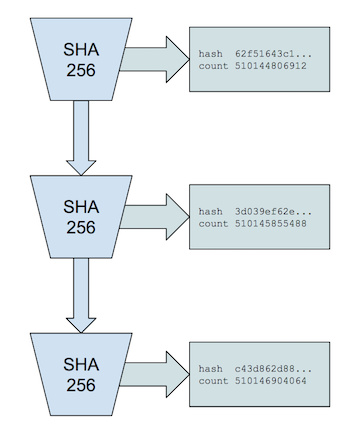
\includegraphics[width=8cm]{images/solana}
    \caption{Schéma simplifié de proof of history}
\end{figure}

On peut y injecter des entrées à tout moment. Cela va changer de manière imprédictible les données futures et ainsi ancrer les données dans l'historique de la chaîne de hachage.

Ce mécanisme a été inventé par Anatoly Yakovenko et est utilisé par la blockchain Solana. Ce protocole est utilisé avant un algorithme de consensus de type \emph{Delegated Byzantine Fault Tolerance}. L'auteur appelle le \emph{Proof of History}: \textbf{Clock before consensus}. C'est-à-dire que le \emph{PoH} ce charges de remettre dans l'ordre les événements avant faire le consensus.

Ce protocole permet d'obtenir une bande passante de transactions très élevée, jusqu'à 50'000 transactions par seconde d'après les créateurs rendant le protocole plus performant que Bitcoin qui atteint lui une douzaine de transactions par secondes.

% TODO: Réécrire Byzantine Fault Tolerance
\subsection{Byzantine Fault Tolerance}

\emph{Byzantine Fault Tolerance} est un large groupe de protocoles permettant d'atteindre un consensus entre les nœuds du réseau en prenant en compte le fait que des nœuds peuvent être indisponibles, transmettre des informations erronées ou être malhonnêtes. Il existe différents types d'algorithme basés sur \emph{BFT} mais la plus part d'entre eux ont un fonctionnement similaire. 

Avec les protocoles \emph{BFT}, pour simplifier, un nœud est choisi pour créer le prochain bloc. Cela peut se faire grâce à un système de vote ou aléatoirement sans tenir compte d'une ressource en particulier. Le bloc est ensuite transmis à travers le réseau à plusieurs autres nœuds. Ces autres nœuds vont faire certaines vérifications et transmettre le bloc à leur tour et le consensus est atteint lorsque la majorité des nœuds a reçu le bloc et est d'accord sur la version de la chaîne de bloc. Ensuite un autre nœud est sélectionné pour le bloc suivant.

Il est facile simple de détecter les fraudes car si les blocs sont invalides ils seront supprimés par les autres nœuds. Cependant les protocoles \emph{BFT} sont pour la plupart vulnérables aux \textbf{attaques de Sybil} donc si une majorité des nœuds du réseau sont malhonnêtes, il sera impossible d'obtenir un consensus correct. C'est pour cela qu'ils sont souvent associer à d'autres protocoles comme \hyperref[consensus:pow]{\emph{PoW}} ou \hyperref[consensus:pos]{\textit{PoS}}.

\section{Analyse des protocoles}

Tous ces protocoles permettent d'une manière ou d'une autre de sécuriser la blockchain. Cependant ils ne respectent pas tous les contraintes écologiques de ce travail. Afin de pouvoir faire un choix, ces protocoles seront ci-dessous analysés afin de pouvoir trouver les mieux adaptés selon différents critères comme l'impact écologique, la facilité d'implémentation, les ressources disponibles et autre points importants.

\begin{itemize}
    \item \textbf{Proof of work}: ce protocole est certes le plus populaire et possède le plus de ressources sur internet, il est cependant le moins écologique de tous. C'est principalement pour cette raison qu'il ne sera pas question d'implémenter un protocole comme \textit{PoW} ou autres protocoles basés sur ce dernier. A noté que l'implémentation d'un algorithme de \textit{proof of work} est plus simple que la majeur partie des autres protocoles.
    \item \textbf{Proof of stake}: écologiquement plus intéressant que PoW, la preuve d'enjeu peut se trouver être une bonne alternative en terme de consommation d'énergie. Cependant, comme elle fonctionne sur le principe de bloquer de l'argent pour la sécurité du réseau, cela implique qu'il faut nécessairement un certaine quantité d'argent dès le début, ce qui est problématique pour commencer une blockchain à partir de rien. \textit{Ethereum} qui effectue une migration de PoW vers PoS possède déjà beaucoup d'argent en circulation pouvant être bloqué pour faire de la preuve d'enjeu convenablement. Mais à partir de rien, c'est conceptuellement difficile ce qui rend l'implémentation plus compliquée.
    \item \textbf{Proof of authority}: PoA est une bonne alternative pour les blockchains privées. Son implémentation est plutôt simple car il n'y a pas besoin d'utiliser des ressources particulières comme de la puissance de calcul, une somme d'argent ou de l'espace de stockage. Il suffit de simplement vérifier les nœuds validateurs qui sont explicitement autorisés par une entité. Il est du coup difficile pour n'importe qui de devenir validateur et contribuer à la sécurité du réseau. C'est pourquoi elle est adaptée à des blockchains privées or, dans ce travail, on souhaite implémenter une cryptomonnaie publique où tout le monde peut contribuer.
    \item \textbf{Proof of space}: ce protocole est intéressant du point de vue énergétique car il fonctionne comme \textit{PoW} mais ne demande pas de puissance de calcule mais de l'espace de stockage à la place. Son empreinte écologique est du coup beaucoup plus faible. Son implémentation est cependant plus complexe car il faut utiliser des graphs permettant de prouver qu'un utilisateur à bien stocker tant de données et ces dernier ne sont pas forcément facile à réaliser. Mais il existe des implémentations de \textit{proof of space} comme Chia ou encore Spacemesh ce qui fournissent déjà un quantité de ressources acceptable. Ce protocole est un très bon candidat pour ce travail car bien adapté.
    \item \textbf{Proof of replication}: ce protocole possède les mêmes avantages que proof of space vue juste au dessus mais avec en plus l'avantage que les données stockées sont des données utiles. Mais en revanche l'implémentation est beaucoup plus compliquée. Prouver qu'un utilisateur à stocker des réplicas de fichiers est plus complexe mathématiquement que de prouver qu'il a stocker des données pseudo-aléatoires. Il y a des ressources comme Filecoin qui sont disponibles et peuvent aider à comprendre le fonctionnement mais cela reste trop de travail pour ce projet.
    \item \textbf{Proof of weight}: étant une famille de protocole, il n'existe pas un protocole mais plusieurs avec par exemple \textit{proof of stake} qui peut être associé à du \textit{proof of weight} d'une certaine manière. En tant que tel, \textit{proof of weight} est assez jeune et très peu utilisé avec peu d'information disponible sur internet, c'est pourquoi il sera mis de côté mais reste un protocole intéressant sachant qu'on peut dériver du \textit{PoSpace} en \textit{PoWeight} en assignant un poids relatif à l'espace de stockage.
    \item \textbf{Proof of importance}: le principe de ce protocole est également intéressant mais est, à nouveau, très jeune avec peu de ressources disponibles. Se lancer dans l'implémentation d'un tel protocole est trop risqué.
    \item \textbf{Proof of burn}: \textit{Proof of burn} a un concept assez spécial et peut être un protocole écologique si les coins brûlé sont les coins de la cryptomonnaie même. Cependant ce protocole n'a jamais été testé à large échelle et se trouve être assez théorique avec très peu d'implémentations existantes et de ressources disponibles le rendant peu attractif.
    \item \textbf{Proof of history}: probablement le protocole le plus intéressant avec \textit{proof of space} car c'est également un protocole plus écologique que \textit{PoW}. Son concept est innovant et utilisé dans la blockchain Solana donc déjà plus ou moins déployé. Cependant les concepts utilisés sont plus obscures que ceux utilisés avec \textit{proof of space} ce qui rend son implémentation plus compliquée car plus difficile à comprendre. Il y a quelques ressources disponible sur la documentation de Solana mais moins que sur le réseau Chia par exemple.
    \item \textbf{Byzantine Fault Tolerance}: cette famille de protocole englobe tous les algorithmes de consensus vu ci-dessus, ce n'est pas un protocole à proprement dit. On utilise un ou plusieurs protocoles vu précédemment pour avoir de la \textit{Byzantine Fault Tolerance} au sein d'un réseau d'ordinateurs distribués. Cela pour éviter principalement les attaques de Sybil.
\end{itemize}

% TODO: Attaque sur les blockchains
\section{Attaques sur les blockchains}

\subsection{Attaque Sybil}

\lipsum[1]

\subsection{Attaque des 51\%}

\lipsum[1]

\subsection{Problème du "Nothing-to-stake"}

\lipsum[1]

\section{Mécanismes de sécurisation}

La technologie de la blockchain apporté par Bitcoin est révolutionnaire. Pouvoir faire des paiements sans passer par un organisme centrale est génial mais le problème pour réaliser cela est qu'il faut conserver publiquement un registre de toutes les transactions. Les entrées et sorties des transactions sont identifiées par des adresses dérivées des clés publiques des utilisateurs. Les transactions sont ainsi pseudonymes. Satoshi Nakamoto l'a dit dans son whitepaper: \textit{The public can see that someone is sending an amount to someone else, but without information linking the transaction to anyone.}

Mais les transaction ne sont pas anonymes. On peut quand même voir le montant, de qui et vers qui va l'argent même si on ne sais pas forcément qui sont derrières les adresses. Il faut bien faire la distinction entre \emph{anonyme} et \emph{pseudonyme}.

Cependant, il existe des blockchains qui permettent d'anonymiser leurs transactions. Rendant illisible le montant et les adresses ainsi que tout autres données. Les deux cryptomonnaies les plus connue à ce sujet sont présentées ci-dessous. 

% TODO: Écrire Zcash
\subsection{Zcash}

\lipsum[1]

% TODO: Écrire Monero
\subsection{Monero}

\lipsum[1]

\section{Cryptomonnaies de 3ème génération}

On peut qualifier le Bitcoin de 1ère génération de cryptomonnaie. Il y a eu ensuite Ethereum et l'apparition des smart-contracts considéré comme cryptomonnaie de 2ème génération. Et maintenant il y a les cryptomonnaies de 3ème génération qui tentent de résoudre les problèmes présents avec le Bicoin et Ethereum. Notamment les soucis de performance et de stockage.

\subsection{Performance des blockchains}

Un point important est la performance des blockchains. Or le Bitcoin ne peut traiter que 4 à 5 transactions par seconde ce qui le rend très peu performant comparé au réseau VISA qui traite environ 2000 transactions par seconde en moyenne et peu monter plus haut en cas de forte affluence. Le problème vient du fait qu'il faut 10 minutes pour générer un bloc et que chaque bloc fait au maximum 1 mégaoctet. Ces informations sont codées en dur dans le code source de Bitcoin ce qui veut dire qu'il est possible de les modifier pour améliorer les performances du réseau Bitcoin. Mais alors pourquoi les développeurs ne l'ont pas fait ? 

Il y a deux possibilités: 1. réduire le temps de génération d'un bloc et 2. augmenter la taille maximum d'un bloc. 

La première possibilité est compliquée à mettre en place car la propagation d'un nouveau bloc à travers le réseau prend du temps. Réduire le temps de création implique de réduire la difficulté de la preuve de travail ce qui fera que plus de mineurs généreront plus de blocs rendant le consensus plus compliqué à cause du nombre de mineurs présent sur le réseau et d'un propagation lente.

La deuxième possibilité à fait de grands débats au sein de la communauté. C'est facile d'augmenter la taille des blocs mais cela implique que la blockchain prendra plus d'espace de stockage à l'avenir. Certains développeurs étaient pour une augmentation et d'autres non ce qui est venu à créer \emph{Bitcoin Cash}, un "hard fork" de Bitcoin. Les développeurs de Bitcoin Cash ont décidé d'augmenter la taille maximum des blocs. Ils ont choisi un bloc dans la blockchain Bitcoin et ont créé une nouvelles branches à partir depuis laquelle les nouveaux blocs de Bitcoin Cash seront créés. Par ailleurs, si vous aviez des Bitcoins avant la séparation vous avez du coup le même montant en Bitcoin Cash (BCH) mais aussi en Bitcoin. Comme les deux branches sont séparées l'une de l'autre, c'est comme si les coins s'étaient dupliqués.

\subsection{Cardano}

% TODO: Écrire Cardano
\lipsum[1]

\subsection{IOTA}

% TODO: Écrire IOTA
\lipsum[1]

\subsection{Solana}

% TODO: Écrire Solana
\lipsum[1]